\section{BouncingBall}
\subsection{Purpose}
This sample was the first non smooth dynamical system simulated with SICONOS platform software.
There's a ball (assimilated to a point) moving on 1 axis.
The ball is falling because of gravity force, and rebounds on a solid floor.

\subsection{results}
We can see on the figure (\ref{fig: BouncingBall}) the position of the moving ball and the position of the floor. Moreover we can see the speed of the ball and the strength of the reaction force when the ball touchs the floor.\\
The bottom axis corresponds to the time, whereas the left axis corresponds to the heigth of the ball.
	\begin{figure}
	\begin{center}
	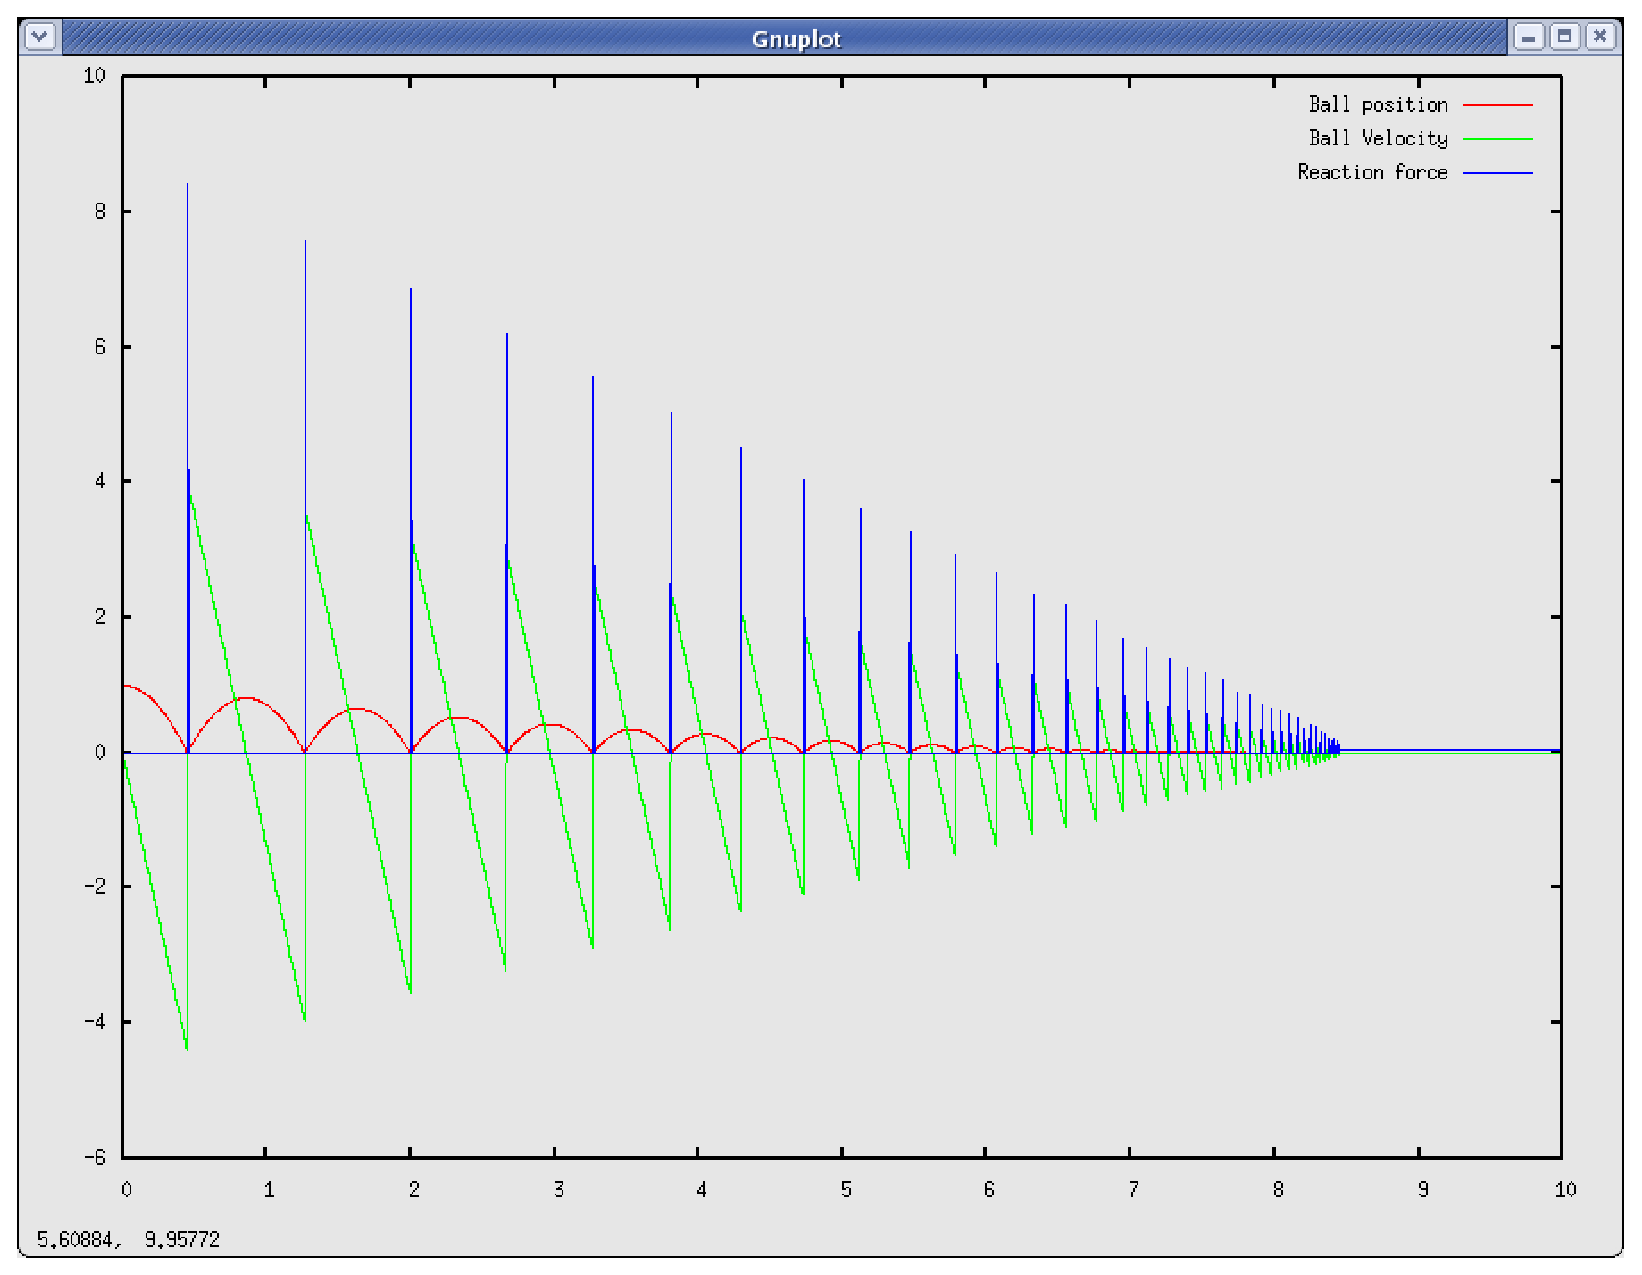
\includegraphics[scale=0.6, clip]{figure/BouncingBall.eps}
	\caption{Evolution of the BouncingBall in relation to the time}
	\label{fig: BouncingBall}
	\end{center}
	\end{figure}

\pagebreak

\section{RollingBalls}
\subsection{Purpose}
This sample has been made to test a non smooth dynamical system with several dynamical systems.\\
There are 3 moving points.\\
All the movements are only on 1 axis!\\
The 3 points are aligned. Each point is moving with different speeds, and will enter in contact with the other points during the simulation.

\subsection{Results}
We can see on the figure (\ref{fig: RollingBalls}) the position of the points and the speed of these points.\\

	\begin{figure}
	\begin{center}
	\includegraphics[scale=0.6, clip]{figure/RollingBalls.eps}
	\caption{Evolution of the RollingBalls in relation to the time}
	\label{fig: RollingBalls}
	\end{center}
	\end{figure}

\pagebreak

\section{DoubleContact}
\subsection{Purpose}
This sample has been made to test multiple contacts between dynamical systems.\\
There are 3 points of which 1 is static, and the 2 others are moving.\\
All the movement are only on 1 axis!\\
The 3 points are aligned. The 2 points that are moving are converging, and the convergence point correponds to the place of the third point.\\
Interactions are defined between points 1 and 2, 2 and 3, 1 and 3. So we have one contact point where the 3 interactions are activated.

\subsection{Results}
We can see on the figure (\ref{fig: DoubleContact}) the position of the points and the speed of these points.\\
When the contact occurs, the moving points are bouncing, changing there direction and losing some speed because of the Newton impact law coefficient (0.9). The middle point don't move because the 2 moving balls hit it with the same speed at the same time.
	\begin{figure}
	\begin{center}
	\includegraphics[scale=0.6, clip]{figure/DoubleContact.eps}
	\caption{Evolution of the DoubleContact balls in relation to the time}
	\label{fig: DoubleContact}
	\end{center}
	\end{figure}

\pagebreak

\section{Ball2D}
\subsection{Purpose}
This sample is the same as the BouncingBall, but this time, the point is moving in 2 dimensions.\\
The point is falling because of gravity force, has an advance velocity, and rebounds on a solid floor.\\

\subsection{Results}
We can see on the figure (\ref{fig: Ball2D}) the height of the point (Y axis) according to his position on the X axis.
	\begin{figure}
	\begin{center}
	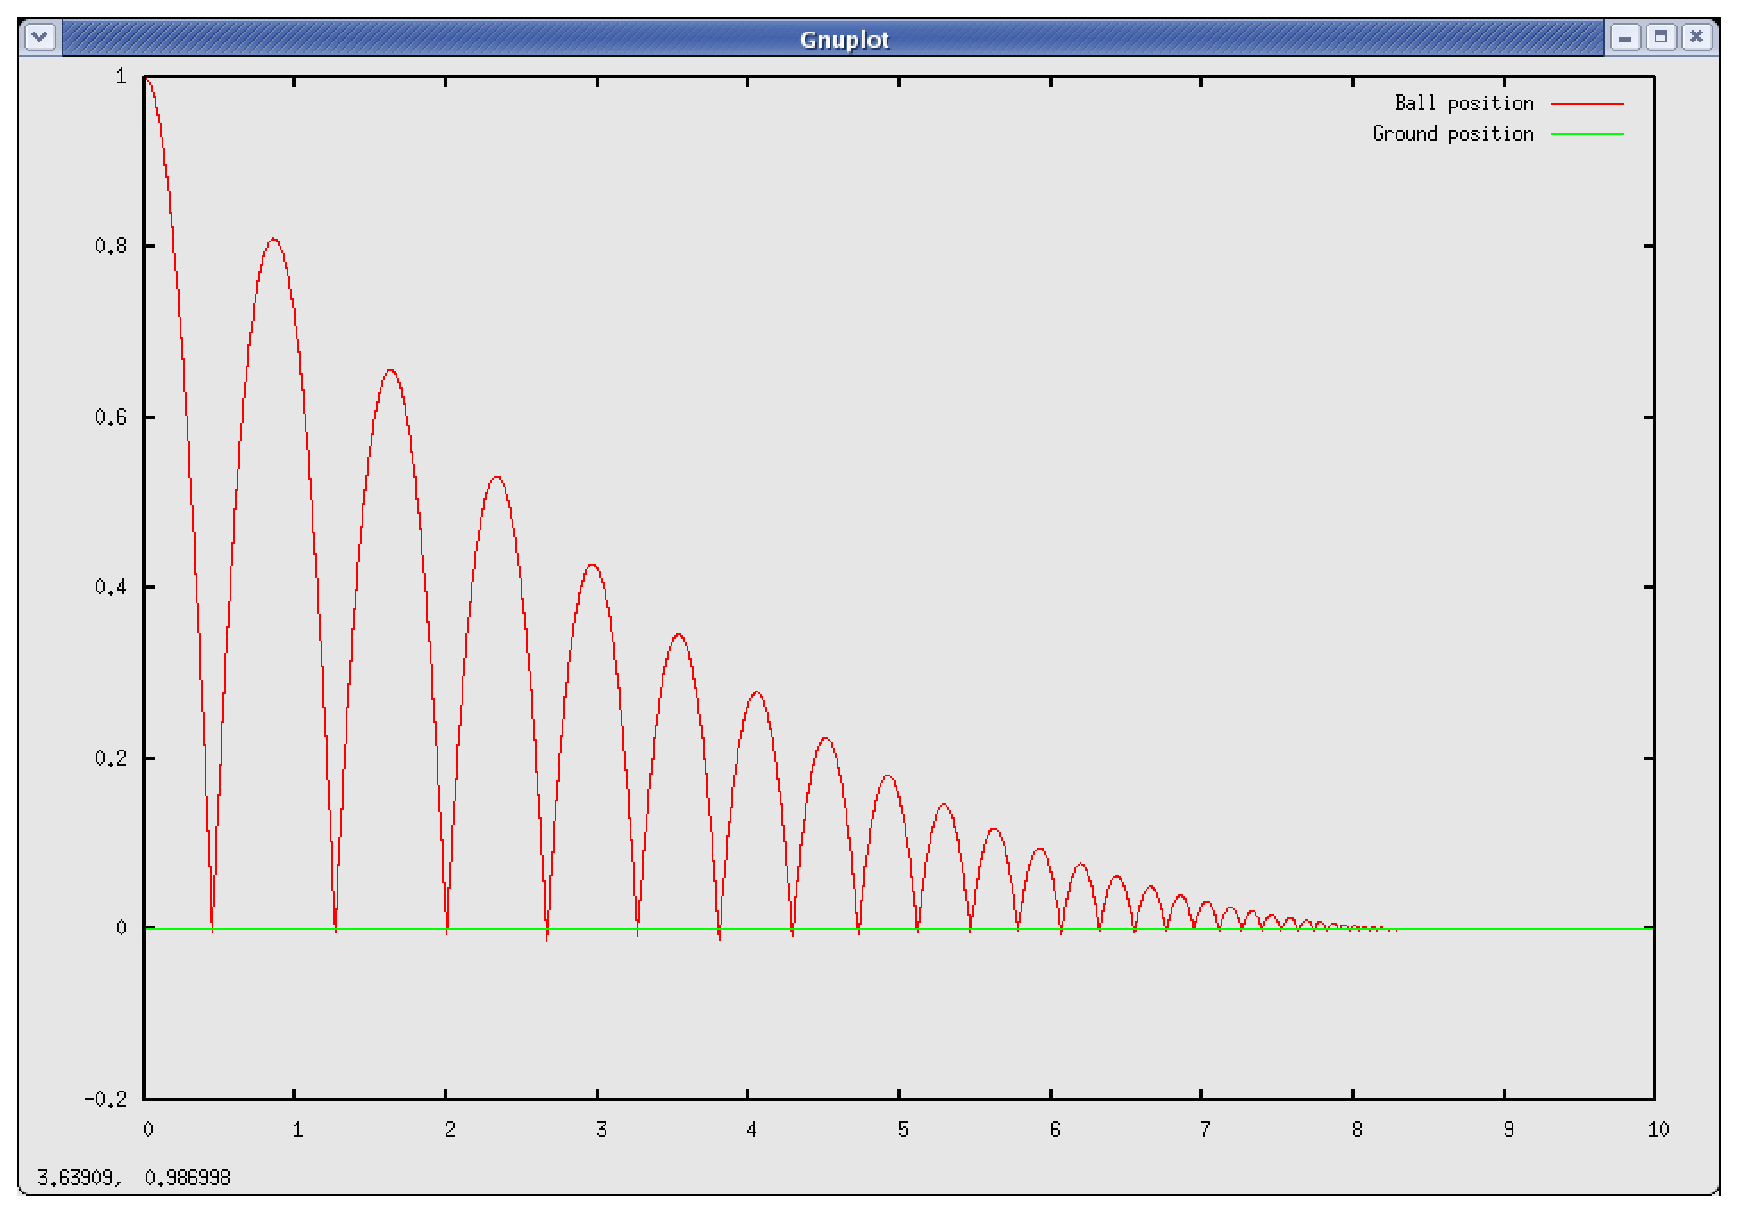
\includegraphics[scale=0.6, clip]{figure/Ball2D.eps}
	\caption{Evolution of the position of a BouncingBall in 2D}
	\label{fig: Ball2D}
	\end{center}
	\end{figure}

\pagebreak

%\section{UltraBalls}
% not yet functionnal
